
\tikzstyle{leaf}=[draw=red!90,fill=red!40,rectangle,thick,minimum height=2.6ex,minimum width=2ex,inner sep=0pt]
\tikzstyle{internal}=[fill=black,circle,inner sep=0pt,minimum size=1ex]

\def\yscale{0.6}
\def\xscale{0.7}

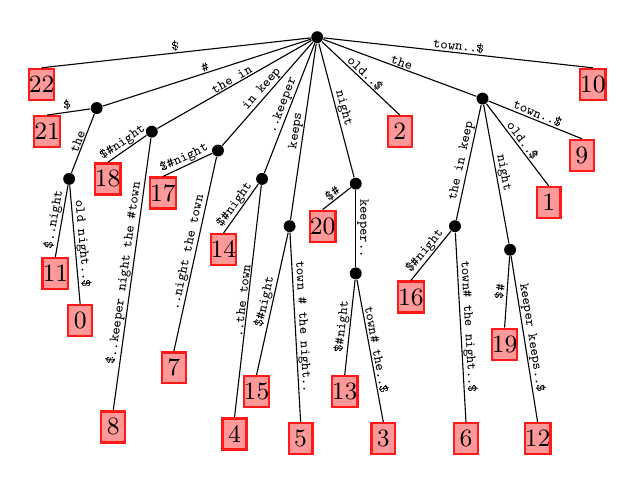
\begin{tikzpicture}
% \draw [help lines] (0,0) grid (10,10);
% \node at (0,0) {(0,0)};
% \node at (10,0) {(10,0)};
% \node at (0,10) {(0,10)};
% \node at (10,10) {(10,10)};

\node[internal] (root) at (5*\xscale,10*\yscale) {};

% children of the root
\node[leaf] (leaf-0) at (0*\xscale,9*\yscale) {\small$22$};
\node[internal] (root-subtree-0) at (1*\xscale,8.5*\yscale) {};
\node[internal] (root-subtree-1) at (2*\xscale,8*\yscale) {};
\node[internal] (root-subtree-2) at (3.2*\xscale,7.6*\yscale) {};
\node[internal] (root-subtree-3) at (4*\xscale,7*\yscale) {};
\node[internal] (root-subtree-4) at (4.5*\xscale,6*\yscale) {};
\node[internal] (root-subtree-5) at (5.7*\xscale,6.9*\yscale) {};
\node[leaf] (leaf-15) at (6.5*\xscale,8*\yscale) {\small$2$};
\node[internal] (root-subtree-6) at (8*\xscale,8.7*\yscale) {};
\node[leaf] (leaf-22) at (10*\xscale,9*\yscale) {\small$10$};

%children of root-subtree-0
\node[leaf] (leaf-1) at (0.1*\xscale,8*\yscale) {\small$21$};
\node[internal] (subtree-0-subtree-1) at (0.5*\xscale,7*\yscale) {};

%children of subtree-0-subtree-1
\node[leaf] (leaf-2) at (0.25*\xscale,5*\yscale) {\small$11$};
\node[leaf] (leaf-3) at (0.7*\xscale,4*\yscale) {\small$0$};

% %children of root-subtree-1
\node[leaf] (leaf-4) at (1.2*\xscale,7*\yscale) {\small$18$};
\node[leaf] (leaf-5) at (1.3*\xscale,1.75*\yscale) {\small$8$};

% %children of root-subtree-2
\node[leaf] (leaf-6) at (2.2*\xscale,6.7*\yscale) {\small$17$};
\node[leaf] (leaf-7) at (2.4*\xscale,3*\yscale) {\small$7$};

% %children of root-subtree-3
\node[leaf] (leaf-8) at (3.3*\xscale,5.5*\yscale) {\small$14$};
\node[leaf] (leaf-9) at (3.5*\xscale,1.6*\yscale) {\small$4$};

% %children of root-subtree-4
%\node[leaf] (leaf-10) at (4.3*\xscale,5.5*\yscale) {\small$20$};
%\node[internal] (subtree-4-subtree-1) at (4.8*\xscale,4*\yscale) {};

% %children of subtree-4-subtree-1
\node[leaf] (leaf-10) at (3.9*\xscale,2.5*\yscale) {\small$15$};
\node[leaf] (leaf-11) at (4.7*\xscale,1.5*\yscale) {\small$5$};

% %children of root-subtree-4
\node[leaf] (leaf-12) at (5.1*\xscale,6*\yscale) {\small$20$};
\node[internal] (subtree-5-subtree-1) at (5.7*\xscale,5*\yscale) {};
\node[leaf] (leaf-13) at (5.5*\xscale,2.5*\yscale) {\small$13$};
\node[leaf] (leaf-14) at (6.2*\xscale,1.5*\yscale) {\small$3$};

% %children of root-subtree-5
% \node[leaf] (leaf-9) at (3.5,2.5*\yscale) {\small$18$};
% \node[internal] (subtree-5-subtree-1) at (4,2*\yscale) {};

% %children of subtree-5-subtree-1
% \node[leaf] (leaf-10) at (3.6,0.5*\yscale) {\small$11$};
% \node[leaf] (leaf-11) at (4.1,0*\yscale) {\small$2$};

% %children of root-subtree-6

\node[internal] (subtree-6-subtree-1) at (7.5*\xscale,6*\yscale) {};
\node[internal] (subtree-6-subtree-2) at (8.5*\xscale,5.5*\yscale) {};
\node[leaf] (leaf-16) at (6.7*\xscale,4.5*\yscale) {\small$16$};
\node[leaf] (leaf-17) at (7.7*\xscale,1.5*\yscale) {\small$6$};

\node[leaf] (leaf-18) at (8.4*\xscale,3.5*\yscale) {\small$19$};
\node[leaf] (leaf-19) at (9*\xscale,1.5*\yscale) {\small$12$};
\node[leaf] (leaf-20) at (9.2*\xscale,6.5*\yscale) {\small$1$};
\node[leaf] (leaf-21) at (9.8*\xscale,7.5*\yscale) {\small$9$};


% edge label mapping
% #           1
% the 1       8
% old 2       7
% night 3     6
% keeper 4    4
% keeps 5     5
% keep 6      3
% in 7        2
% town 8      9
% 
% # 
% 1876458328918645832861

% edges from root to children
\draw (root) -- (leaf-0.north)  node [midway,above=-3pt,sloped] {\tiny \tt \$};
\draw (root) -- (root-subtree-0)  node [sloped,midway,above=-3pt] {\tiny \tt \#};
\draw (root) -- (root-subtree-1)  node [sloped,midway,above=-3pt] {\tiny \tt the in};
\draw (root) -- (root-subtree-2)  node [sloped,midway,above=-3pt] {\tiny \tt in keep};
\draw (root) -- (root-subtree-3)  node [sloped,midway,above=-3pt] {\tiny \tt ..keeper};
\draw (root) -- (root-subtree-4)  node [sloped,midway,above=-3pt] {\tiny \tt keeps};
\draw (root) -- (root-subtree-5)  node [sloped,midway,above=-3pt] {\tiny \tt night};
\draw (root) -- (leaf-15.north)  node [sloped,midway,above=-3pt] {\tiny \tt old..\$};
\draw (root) -- (root-subtree-6)  node [sloped,midway,above=-3pt] {\tiny \tt the};
\draw (root) -- (leaf-22.north)  node [midway,above=-3pt,sloped] {\tiny \tt town..\$};

% edges from root-subtree-1 to children
\draw (root-subtree-0) -- (leaf-1.north)  node [midway,above=-3pt,sloped] {\tiny \tt \$};
\draw (root-subtree-0) -- (subtree-0-subtree-1)  node [midway,above=-3pt,sloped] {\tiny \tt the};

% edges from subtree-0-subtree-1 to children
\draw (subtree-0-subtree-1) -- (leaf-2.north)  node [midway,above=-3pt,sloped] {\tiny \tt \$..night};
\draw (subtree-0-subtree-1) -- (leaf-3.north)  node [sloped,midway,above=-3pt] {\tiny \tt old night..\$};

% % edges from root-subtree-1 to children
\draw (root-subtree-1) -- (leaf-4.north)  node [midway,above=-3pt,sloped] {\tiny \tt \$\#night};
\draw (root-subtree-1) -- (leaf-5.north)  node [midway,above=-3pt,sloped] {\tiny \tt \$..keeper night the \#town};

% % edges from root-subtree-2 to children
\draw (root-subtree-2) -- (leaf-6.north)  node [midway,above=-3pt,sloped] {\tiny \tt \$\#night};
\draw (root-subtree-2) -- (leaf-7.north)  node [midway,above=-3pt,sloped] {\tiny \tt ..night the town};

% % edges from root-subtree-3 to children
\draw (root-subtree-3) -- (leaf-8.north)  node [midway,above=-3pt,sloped] {\tiny \tt \$\#night};
\draw (root-subtree-3) -- (leaf-9.north)  node [midway,above=-3pt,sloped] {\tiny \tt ..the town};

% % edges from root-subtree-4 to children
%\draw (root-subtree-4) -- (leaf-10.north)  node [midway,above=-3pt,sloped] {\tiny \tt \$\#};
%\draw (root-subtree-4) -- (subtree-4-subtree-1)  node [midway,above=-3pt,sloped] {\tiny \tt the in keep the};

% % edges from root-subtree-4 to children
\draw (root-subtree-4) -- (leaf-10.north)  node [midway,above=-3pt,sloped] {\tiny \tt \$\#night};
\draw (root-subtree-4) -- (leaf-11.north)  node [sloped,midway,above=-3pt] {\tiny \tt town \# the night..};

% % edges from subtree-5-subtree-1 to children
\draw (root-subtree-5) -- (leaf-12.north)  node [midway,above=-3pt,sloped] {\tiny \tt \$\#};
\draw (root-subtree-5) -- (subtree-5-subtree-1)  node [midway,above=-3pt,sloped] {\tiny \tt keeper..};
\draw (subtree-5-subtree-1) -- (leaf-13.north)  node [midway,above=-3pt,sloped] {\tiny \tt \$\#night};
\draw (subtree-5-subtree-1) -- (leaf-14.north)  node [sloped,midway,above=-3pt] {\tiny \tt town\# the..\$};


% % edges from root-subtree-6 to children
% \draw (root-subtree-6) -- (leaf-17.north)  node [sloped,midway,above=-3pt] {\tiny \tt old..\$};
% \draw (root-subtree-6) -- (leaf-18.north)  node [sloped,midway,above=-3pt] {\tiny \tt town..\$};
\draw (root-subtree-6)  -- (subtree-6-subtree-1)  node [sloped,midway,above=-3pt] {\tiny \tt the in keep};
\draw (root-subtree-6)  -- (subtree-6-subtree-2)  node [sloped,midway,above=-3pt] {\tiny \tt night};
\draw (subtree-6-subtree-2) -- (leaf-18.north)  node [midway,above=-3pt,sloped] {\tiny \tt \$\#};
\draw (subtree-6-subtree-2) -- (leaf-19.north)  node [midway,above=-3pt,sloped] {\tiny \tt keeper keeps..\$};
\draw (root-subtree-6) -- (leaf-20.north)  node [midway,above=-3pt,sloped] {\tiny \tt old..\$};
\draw (root-subtree-6) -- (leaf-21.north)  node [midway,above=-3pt,sloped] {\tiny \tt town..\$};
% \draw (root-subtree-6)  -- (subtree-6-subtree-2)  node [sloped,midway,above=-3pt] {\tiny \tt night};

% % edges from root-subtree-subtree-6-subtree-1 to children
\draw (subtree-6-subtree-1)  -- (leaf-16.north)  node [sloped,midway,above=-3pt] {\tiny \tt \$\#night};
\draw (subtree-6-subtree-1)  -- (leaf-17.north)  node [sloped,midway,above=-3pt] {\tiny \tt town\# the night..\$};


% % edges from root-subtree-subtree-6-subtree-2 to children
% \draw (subtree-6-subtree-2)  -- (leaf-15.north)  node [sloped,midway,above=-3pt] {\tiny \tt \$};
% \draw (subtree-6-subtree-2)  -- (leaf-16.north)  node [sloped,midway,above=-3pt] {\tiny \tt keeper..\$};


\end{tikzpicture}